
\chapter{Hybrid Finite Volume Methods}
\label{chp:HFVMMethod}
%Framework of methods

%Elliptic Equations
%	FD(3rd order)
% 	FEM(3rd and 2nd order, mention matrix solvers)

%Conservation Law
% 	3rd order, 2nd order (modifications)

%Cell average to Nodal vales

%RK Steps

%B.C/ Dry Solution / Well balancing (already in Hons thesis)

%Grid Definition

\section{Structure Overview}

%Define how these arrays are constructed, also use u at the edges

In this section we will give the general structure for how the hybrid finite volume methods take the array of cell average values at time $t^n$; $\bar{\boldsymbol{h}}^n$ and $\bar{\boldsymbol{G}}^n$ and evolve the system to the cell average values at time $t^{n+1}$; $\bar{\boldsymbol{h}}^{n+ 1}$ and $\bar{\boldsymbol{G}}^{n+ 1}$.

\begin{itemize}
	\item The cell average values are transformed into nodal values by $\mathcal{M}$
		\newline  \centering $\bar{\boldsymbol{h}}^n, \bar{\boldsymbol{G}}^n  \xrightarrow{\mathcal{M}}  \boldsymbol{h}^n, \boldsymbol{G}^n  $ 
    \item $\boldsymbol{u}^n$ is found by solving the elliptic equation in Def. \ref{defn:SerreEqnConservedQuantity1} by $\mathcal{A}$
   		\newline   \centering ${\boldsymbol{h}}^n, {\boldsymbol{G}}^n , {\boldsymbol{b}}  \xrightarrow{\mathcal{\mathcal{G}}}  \boldsymbol{u}^n  $
	\item The conservation equations \eqref{eqn:FullSerreCon} can now be solved by $\mathcal{F}$ 
		\newline   \centering $\bar{\boldsymbol{h}}^n, \bar{\boldsymbol{G}}^n, {\boldsymbol{b}}, {\boldsymbol{u}}^n  \xrightarrow{\mathcal{\mathcal{F}}}  \bar{\boldsymbol{h}}^{n+ 1}, \bar{\boldsymbol{G}}^{n+ 1}  $
\end{itemize}

\begin{defn}
	\label{defn:EulerStep}
	$\mathcal{E}$ is the single Euler step given by the procedure above that transforms updates the array of cell average values at time $t^n$; $\bar{\boldsymbol{h}}^n$ and $\bar{\boldsymbol{G}}^n$ to the cell average values at time $t^{n+1}$; $\bar{\boldsymbol{h}}^{n+ 1}$.
	$$\bar{\boldsymbol{h}}^n, \bar{\boldsymbol{G}}^n,  {\boldsymbol{b}} \xrightarrow{\mathcal{\mathcal{E}}}  \bar{\boldsymbol{h}}^{n+ 1}, \bar{\boldsymbol{G}}^{n+ 1}  $$
\end{defn}

\section{Transformation Between Nodal Values and Cell Averages}
For first and second order methods $\mathcal{M}$ is just the identity map as the cell average values are equal to the nodal values.

For higher order methods this is not the case, hence why there is a need to incorporate the process $\mathcal{M}$ into our methods, as assuming that $\mathcal{M}$ is the identity map will lead to a loss of accuracy in the method. 

From quadratic interpolation we have the formula relating the cell averages and nodal values of a quantity  $q$ with third order accuracy

\begin{equation*}
q_j = \frac{-\bar{q}_{j- 1} + 26\bar{q}_{j} - \bar{q}_{j + 1}}{24}.
\end{equation*}

Therefore 

\begin{equation*}
\boldsymbol{q} = \frac{1}{24}
\begin{bmatrix}
26  & -1  & & & \\
-1  & 26  & -1  &  & \\
 & \ddots & \ddots &  \ddots & \\
  &  & -1 & 26  &  -1\\
 &   &  & -1 & 26  \\
\end{bmatrix}
 \bar{\boldsymbol{q}}.
\end{equation*}

Dirichlet boundary conditions at edges.

So for the third-order method $\mathcal{M}$ is a multiplication by the above matrix. 

\section{Elliptic Equation}
The elliptic equation that relates the conserved variables $h$ and $G$ to the primitive variable $u$ was given in Def \ref{defn:SerreEqnConservedQuantity1} and is presented here to remind the reader

	\[ G =  uh \left(1 + \frac{\partial h}{\partial x}\frac{\partial b}{\partial x} + \frac{1}{2}h\frac{\partial^2 b}{\partial x^2} + \frac{\partial b}{\partial x}^2 \right) - \frac{\partial}{\partial x}\left(\frac{1}{3}h^3  \frac{\partial {u}}{\partial x}\right).\]
\subsection{Finite Difference Methods}
One way to approximate this ordinary differential equation is to replace all the derivatives with finite differences as has been done to second order accuracy in []. We have expanded this work by  building a fourth order accurate finite difference method, where all derivatives were replaced with their centred fourth order approximation. This results in the following equation for each row of a the matrix $\boldsymbol{A}$

\begin{equation}
G_j = A_{j,j-2} \;u_{j-2} + A_{j,j-1} \; u_{j-1} + A_{j,j} \; u_{j} +  A_{j,j + 1} \;u_{j+1} +  A_{j,j + 2} \;u_{j+2}
\end{equation}

where 

\begin{align*}
&A_{j,j-2} = -h^2_j \left(\frac{h_{j-2}  - 8h_{j-1}  + 8 h_{j+1} -h_{j+2} }{144 \Delta x ^2}\right) + \frac{h_{j}^3}{36 \Delta x^2} , \\
&A_{j,j-1} = h^2_j \left(\frac{h_{j-2}  - 8h_{j-1}  + 8 h_{j+1} -h_{j+2}}{18 \Delta x ^2}\right) - \frac{4h_{j}^3}{9 \Delta x^2} , \\
&A_{j,j} = h_j + \frac{5h_{j}^3}{6 \Delta x^2}   + h_j \left(\frac{ \left(h_{j-2}  - 8h_{j-1}  + 8 h_{j+1} -h_{j+2} \right) \left(b_{j-2}  - 8b_{j-1}  + 8 b_{j+1} -b_{j+2} \right) }{144 \Delta x ^2}\right)  \\
& \hspace{1cm}+ h_j \left(\frac{-b_{j-2} + 16 b_{j-1} - 30b_{j-1} + 16b_{j+1} - b_{j+2}}{24 \Delta x ^2}\right)  + h_j \left(\frac{b_{j-2}  - 8b_{j-1}  + 8 b_{j+1} -b_{j+2} }{144 \Delta x ^2}\right), \\ 
&A_{j,j+1} = -h^2_j \left(\frac{h_{j-2}  - 8h_{j-1}  + 8 h_{j+1} -h_{j+2} }{18 \Delta x ^2}\right) - \frac{4h_{j}^3}{9 \Delta x^2} , \\
&A_{j,j+2} = h^2_j \left(\frac{h_{j-2}  - 8h_{j-1}  + 8 h_{j+1} -h_{j+2} }{144 \Delta x ^2}\right) + \frac{h_{j}^3}{36 \Delta x^2} , \\
\end{align*}

This can be written for the whole domain 

\begin{equation*}
\boldsymbol{G} = \boldsymbol{A}
\boldsymbol{u}.
\end{equation*}
Dirichlet boundary conditions

Therefore $\mathcal{G}$ is the solution of this matrix problem with $\boldsymbol{G}$ known and $\boldsymbol{u}$ unknown. 

For completeness the second-order method finite difference approximation which is used for both the first and second order FDVM [] is given by

\begin{equation*}
G_j = A_{j,j-1} \; u_{j-1} + A_{j,j} \; u_{j} +  A_{j,j + 1} \;u_{j+1}
\end{equation*}

where 
\begin{align*}
&A_{j,j-1} = h^2_j\frac{-h_{j-1} + h_{j+1}}{4 \Delta x ^2} - \frac{h_{j}^3}{3 \Delta x ^2}, \\
&A_{j,j} = h_j + h_j \frac{-h_{j-1} + h_{j+1}}{2 \Delta x}\frac{-b_{j-1} + b_{j+1}}{2 \Delta x} + h_j^2\frac{b_{j-1} - 2b_j + b_{j+1}}{2 \Delta x^2} + h_j \left(\frac{-b_{j-1} + b_{j+1}}{2 \Delta x}\right)^2 \\
& \hspace{1cm}+ \frac{2 h_j^3}{3 \Delta x^2}, \\ \\
&A_{j,j+1} = -h^2_j\frac{-h_{j-1} + h_{j+1}}{4 \Delta x ^2} - \frac{h_{j}^3}{3 \Delta x ^2}. \\
\end{align*}

\subsection{Finite Element Methods}
For a finite element method we take the weak form of the elliptic equation in Def \ref{defn:SerreEqnConservedQuantity1} which is 

	\[ \int_{\Omega } G v \; dx =  \int_{\Omega } uh \left(1 + \frac{\partial h}{\partial x}\frac{\partial b}{\partial x} + \frac{1}{2}h\frac{\partial^2 b}{\partial x^2} + \frac{\partial b}{\partial x}^2 \right) - \frac{\partial}{\partial x}\left(\frac{1}{3}h^3  \frac{\partial {u}}{\partial x}\right) v \; dx.\]
	
Which after rearranging, using integration by parts and assuming Dirichlet boundary conditions becomes

%\begin{multline}
%\int_{\Omega } G v \; dx = + \int_{\Omega } uh \left(1 + \frac{\partial b}{\partial x}^2 \right) v \; dx +  %\int_{\Omega } \frac{1}{3}h^3  \frac{\partial {u}}{\partial x} \frac{\partial v}{\partial x} \; dx  \\ + 
%\int_{\Omega }  \frac{\partial }{\partial x} \left(\frac{1}{2}h^2\frac{\partial b}{\partial x}\right) u v \; %dx.
%\end{multline}

%\begin{multline}
%\int_{\Omega } G v \; dx = + \int_{\Omega } uh \left(1 + \frac{\partial b}{\partial x}^2 \right) v \; dx +  %\int_{\Omega } \frac{1}{3}h^3  \frac{\partial {u}}{\partial x} \frac{\partial v}{\partial x} \; dx  \\ - 
%\int_{\Omega }   \frac{1}{2}h^2\frac{\partial b}{\partial x}  \frac{\partial }{\partial x}\left(u v %\right)\; dx.
%\end{multline}

\begin{multline*}
\int_{\Omega } G v \; dx = \int_{\Omega } uh \left(1 + \frac{\partial b}{\partial x}^2 \right) v \; dx +  \int_{\Omega } \frac{1}{3}h^3  \frac{\partial {u}}{\partial x} \frac{\partial v}{\partial x} \; dx  \\ - 
\int_{\Omega }   \frac{1}{2}h^2\frac{\partial b}{\partial x} u \frac{\partial v }{\partial x}\; dx. - 
\int_{\Omega }   \frac{1}{2}h^2\frac{\partial b}{\partial x}  \frac{\partial u }{\partial x}v \; dx.
\end{multline*}
Should be able to handle non smooth $h$ and $G$ but requires first derivative of $b$. We can simplify this further by only performing integration over elements and then assemble them together to get the integral equation for the entire domain. As we use a finite volume method to solve the conservation equations [] our natural element choice are the cells $\left[x_{j-1/2},x_{j+1/2}\right]$. Therefore we get that

\begin{multline}
\label{eq:elementwiseint}
 \sum_{j}  \int_{x_{j-1/2} }^{{x_{j+1/2}}} \Bigg[  \left( uh \left(1 + \frac{\partial b}{\partial x}^2 \right)  - \frac{1}{2}h^2\frac{\partial b}{\partial x}  \frac{\partial u }{\partial x}  -  G \right) v   \\ +  \left( \frac{1}{3}h^3  \frac{\partial {u}}{\partial x}    -     \frac{1}{2}h^2\frac{\partial b}{\partial x} u    \right) \frac{\partial v }{\partial x} \Bigg]dx  = 0.
\end{multline}

for each test function $v$. The next step is to replace the functions for the quantities $h$, $G$, $b$ and $u$ as well as the test function $v$ with the appropriate order of accuracy piece-wise polynomial function. This is typically done using basis functions and this process turns our integral equations into matrix equations.

\subsubsection{Second Order}
We desire a method for the elliptic equation [] that is at least second-order and that can locally reconstruct the necessary physical quantities to update the evolution equations [] within each cell individually. This allows the scheme to be simply scaled into situations where nearby cell data may not be quickly accessible such as when using this method on parrallel cpus. From our equations and smoothness conditions we know that if the bed is smooth enough, then we can allow discontinuous $h$ and $G$ and have $u$ have a well defined derivative. Since in the evolution equations we do not require derivatives of these quantities for $h$ and $G$ we will use linear reconstruction that is discontinuous at the edges for $h$ and $G$ in our finite element method. The basis functions for this reconstruction of $h$ and $G$ will be represented by $\psi$. This reconstruction will use cell values at the edges $x_{j-1/2}$ and $x_{j + 1/2}$ to represent the linear function over the cell.

\begin{figure}
	\centering
	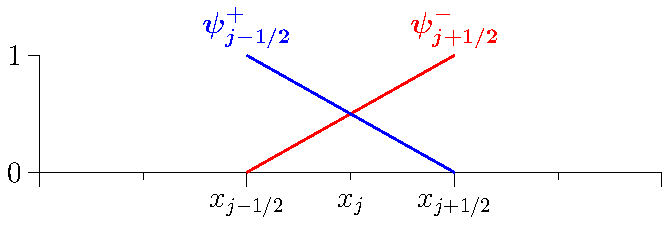
\includegraphics[width=0.8\textwidth]{./chp3/figures/P1.pdf}
	\caption{Basis functions for discontinuous linear elements.}
	\label{fig:P1DiscBasis}
\end{figure}


So we have the following representation for $h$ and $G$ in our finite element method

\begin{align*}
h &= \sum_j h^+_{j-1/2}\psi^+_{j-1/2}  + h^-_{j+1/2}\psi^-_{j+1/2} \\
G &= \sum_j G^+_{j-1/2}\psi^+_{j-1/2}  + G^-_{j+1/2}\psi^-_{j+1/2}
\end{align*}

Where we calculate $h^+_{j-1/2}$, $h^-_{j+1/2}$, $G^+_{j-1/2}$ and $G^-_{j+1/2}$ using our second-order reconstruction. Which for our method is the generalised minmod limiter of \cite{vanLeer-B-1979-101}, which for a general quantity $q$ is
\begin{subequations}
	\begin{gather}
	q^-_{j + 1/2} =  q_j + a_j \dfrac{\Delta x}{2}
	\end{gather}
	and
	\begin{gather}
	q^+_{j + 1/2} =  q_{j+1} - a_{j + 1} \dfrac{\Delta x}{2}
	\end{gather}
	where
	\begin{gather}
	a_j = \text{minmod}\left\lbrace\theta \dfrac{- q_j + q_{j+1}}{\Delta x}, \dfrac{- q_{j-1} + q_{j+1}}{2\Delta x} ,\theta \dfrac{ - q_{j-1} + q_j}{\Delta x}\right\rbrace \quad \text{for} \; \theta \in \left[1,2\right]
	\end{gather}
\end{subequations}



For the velocity term our FVM requires a local second-order approximation of the first derivative. To do this will require a quadratic representation of $u$ in each cell. Since $u$ is guaranteed to have continuous representation across the cells we use a quadratic reconstruction that is continuous at the cell edges. The basis functions for this reconstruction of $u$ will be represented by $\phi$. We will also use these basis functions as our test functions $v$.  This reconstruction will use cell values at $x_{j-1/2}$, $x_{j}$ and $x_{j + 1/2}$ to represent the quadratic function over the cell. 

\begin{figure}
	\centering
	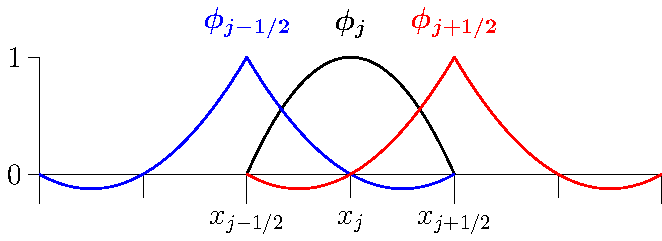
\includegraphics[width=0.8\textwidth]{./chp3/figures/P2.pdf}
	\caption{Basis functions for continuous piecewise quadratic elements.}
	\label{fig:P2ContBasis}
\end{figure}

\begin{equation}
u = \sum_j u_{j-1/2}\phi_{j-1/2} + u_{j}\phi_{j} + u_{j+1/2}\phi_{j+1/2}
\end{equation}

Since we calculate $u$ from the other quantities we do not require a reconstruction scheme for $u_{j-1/2}$, $u_j$ and $u_{j+1/2}$.



For the bed term our FVM requires a second-order approximation of the second derivative of the bed terms that must be done locally. To do this we will require a cubic representation of the bed in each cell. Since by our smoothness conditions we do not allow for discontinuous beds, we will assume the bed is continuous. Therefore we will use a cubic reconstruction for the bed which is continuous across the cell edges. The basis functions for this reconstruction of $b$ will be represented by $\gamma$. This reconstruction will use cell values at $x_{j-1/2}$, $x_{j-1/6}$, $x_{j+1/6}$ and $x_{j + 1/2}$ to represent the cubic function over the cell. 


\begin{figure}
	\centering
	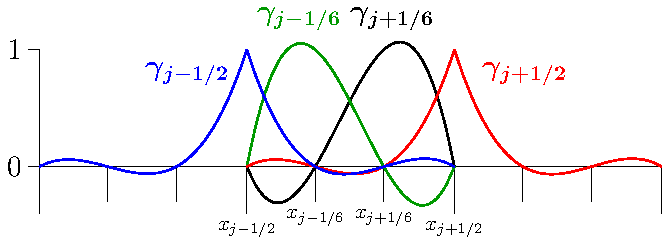
\includegraphics[width=0.8\textwidth]{./chp3/figures/P3.pdf}
	\caption{Basis functions for continuous piecewise cubic elements.}
	\label{fig:P3ContBasis}
\end{figure}

\begin{equation}
b = \sum_j b_{j-1/2}\gamma_{j-1/2} + b_{j-1/6}\gamma_{j-1/6}  + b_{j+1/6}\gamma_{j+1/6} + b_{j+1/2}\gamma_{j+1/2}
\end{equation}

The values $b_{j-1/2}$, $b_{j-1/6}$, $b_{j+1/6}$  and $b_{j+1/2}$ are reconstructed from the cubic that passes through the nodal values $b_{j-2}$, $b_{j-1}$, $b_{j+1}$  and $b_{j+2}$. Which is given by

\begin{multline}
Q^b_j(x)= \frac{-b_{j-2} +2 b_{j-1} - 2 b_{j+1} + b_{j+2}}{12\Delta x^3} \left(x - x_j\right)^3 \\ +  \frac{b_{j-2} - b_{j-1} - b_{j+1} + b_{j+2}}{6\Delta x^2} \left(x - x_j\right)^2 +  \frac{b_{j-2} - 8b_{j-1} +8 b_{j+1} - b_{j+2}}{12\Delta x} \left(x - x_j\right) \\ + \frac{-b_{j-2} + 4b_{j-1} + 4 b_{j+1} - b_{j+2}}{6}
\end{multline}

then we have the following

\begin{align*}
b_{j-1/2} & = Q^b_j(x_{j-1/2}) \\
b_{j-1/6} & = Q^b_j(x_{j-1/6}) \\
b_{j+1/6} & = Q^b_j(x_{j+1/6}) \\
b_{j+1/2} & = Q^b_j(x_{j+1/2}). 
\end{align*}

\subsubsection{Element wise}
Since the integral equation \eqref{eq:elementwiseint} must be true for all $v$, in particular it must hold for $\phi_{j-1/2}$, $\phi_{j}$ and $\phi_{j+1/2}$. Since only these basis functions are non-zero over the element $\left[x_{j-1/2}, x_{j+1/2}\right]$, we can calculate the $j$th term in the sum \eqref{eq:elementwiseint} completely like so

\begin{multline}
\int_{x_{j-1/2} }^{{x_{j+1/2}}} \Bigg[  \left( uh \left(1 + \frac{\partial b}{\partial x}^2 \right)  - \frac{1}{2}h^2\frac{\partial b}{\partial x}  \frac{\partial u }{\partial x}  -  G \right) \begin{bmatrix}
\phi_{j-1/2}\\\phi_j \\\phi_{j+1/2}
\end{bmatrix}   \\ +  \left( \frac{1}{3}h^3  \frac{\partial {u}}{\partial x}    -     \frac{1}{2}h^2\frac{\partial b}{\partial x} u    \right) \frac{\partial}{\partial x}\left(\begin{bmatrix}
\phi_{j-1/2}\\\phi_j \\\phi_{j+1/2}
\end{bmatrix} \right) \Bigg]dx
\end{multline}

where we use our finite element approximations for $h$, $u$, $G$ and $b$. Because our basis functions over one element are just translations of the the other basis functions, this integral can be generalised by moving to what is commonly called the $\xi$ space. For our current definitions the mapping from the $x$ space to the $\xi$ space is

\begin{equation*}
x = x_j + \xi \frac{\Delta x}{2}
\end{equation*}

Making the change of variables the integral becomes

\begin{multline}
\frac{\Delta x}{2}\int_{-1 }^{1} \Bigg[  \left( uh \left(1 + \frac{4}{\Delta x^2}\frac{\partial b}{\partial \xi}^2 \right)  - \frac{1}{2}h^2  \frac{4}{\Delta x^2} \frac{\partial b}{\partial \xi}  \frac{\partial u }{\partial \xi}  -  G \right) \begin{bmatrix}
\phi_{j-1/2}\\\phi_j \\\phi_{j+1/2}
\end{bmatrix}   \\ +  \left( \frac{1}{3}h^3 \frac{2}{\Delta x}\frac{\partial {u}}{\partial \xi}    -     \frac{1}{2}h^2 \frac{2}{\Delta x}\frac{\partial b}{\partial \xi} u    \right)  \frac{2}{\Delta x}\frac{\partial}{\partial \xi}\left(\begin{bmatrix}
\phi_{j-1/2}\\\phi_j \\\phi_{j+1/2}
\end{bmatrix} \right) \Bigg]d\xi
\end{multline}

where all functions have $\xi$ as there variable instead of $x$. We will now demonstrate the rest of this process for the term $uh$ and then give the remaining matrices. Focusing on the $uh$ term we have to compute  

\begin{equation}
\frac{\Delta x}{2}\int_{-1 }^{1}  uh \begin{bmatrix}
\phi_{j-1/2}\\\phi_j \\\phi_{j+1/2}
\end{bmatrix} d\xi
\end{equation}

Since we are computing the integral over $\left[x_{j-1/2},x_{j+1/2}\right]$ the only non-zero contributions from the finite element approximation to $h$ and $u$ are


\begin{equation}
\frac{\Delta x}{2}\int_{-1 }^{1}  \left(u_{j-1/2}\phi_{j-1/2} + u_{j}\phi_{j} + u_{j+1/2}\phi_{j+1/2}\right) \left(h^+_{j-1/2}\psi^+_{j-1/2}  + h^-_{j+1/2}\psi^-_{j+1/2}\right) \begin{bmatrix}
\phi_{j-1/2}\\\phi_j \\\phi_{j+1/2}
\end{bmatrix} d\xi
\end{equation}

\begin{equation}
\frac{\Delta x}{2}\int_{-1 }^{1}  \begin{bmatrix}
\phi_{j-1/2} &\phi_j  &\phi_{j+1/2}
\end{bmatrix} \begin{bmatrix}
u_{j-1/2}\\u_j \\u _{j+1/2}
\end{bmatrix} \left(h^+_{j-1/2}\psi^+_{j-1/2}  + h^-_{j+1/2}\psi^-_{j+1/2}\right) \begin{bmatrix}
\phi_{j-1/2}\\\phi_j \\\phi_{j+1/2}
\end{bmatrix} d\xi
\end{equation}

\begin{equation}
\left(\frac{\Delta x}{2}\int_{-1 }^{1} \left(h^+_{j-1/2}\psi^+_{j-1/2}  + h^-_{j+1/2}\psi^-_{j+1/2}\right) \begin{bmatrix}
\phi_{j-1/2} \phi_{j-1/2} & \phi_{j}  \phi_{j-1/2}  & \phi_{j+1/2} \phi_{j-1/2}\\\phi_{j-1/2} \phi_{j} & \phi_{j} \phi_{j} &  \phi_{j + 1/2} \phi_{j}\\\phi_{j+1/2} \phi_{j-1/2} &  \phi_{j+1/2} \phi_{j} & \phi_{j+1/2} \phi_{j+1/2}
\end{bmatrix} d\xi \right) \begin{bmatrix}
u_{j-1/2}\\u_j \\u _{j+1/2}
\end{bmatrix}
\end{equation}

\begin{multline}
\frac{\Delta x}{2}\Bigg( h^+_{j-1/2} \int_{-1 }^{1} \psi^+_{j-1/2}  \begin{bmatrix}
\phi_{j-1/2} \phi_{j-1/2} & \phi_{j}  \phi_{j-1/2}  & \phi_{j+1/2} \phi_{j-1/2}\\\phi_{j-1/2} \phi_{j} & \phi_{j} \phi_{j} &  \phi_{j + 1/2} \phi_{j}\\\phi_{j+1/2} \phi_{j-1/2} &  \phi_{j+1/2} \phi_{j} & \phi_{j+1/2} \phi_{j+1/2}
\end{bmatrix} d\xi  \\  h^-_{j+1/2}\int_{-1 }^{1} \psi^-_{j+1/2} \begin{bmatrix}
\phi_{j-1/2} \phi_{j-1/2} & \phi_{j}  \phi_{j-1/2}  & \phi_{j+1/2} \phi_{j-1/2}\\\phi_{j-1/2} \phi_{j} & \phi_{j} \phi_{j} &  \phi_{j + 1/2} \phi_{j}\\\phi_{j+1/2} \phi_{j-1/2} &  \phi_{j+1/2} \phi_{j} & \phi_{j+1/2} \phi_{j+1/2}
\end{bmatrix} d\xi \Bigg) \\  \begin{bmatrix}
u_{j-1/2}\\u_j \\u _{j+1/2}
\end{bmatrix}
\end{multline}

Calculating these integrals we get that

\begin{multline}
\frac{\Delta x}{2}\int_{-1 }^{1}  uh \begin{bmatrix}
\phi_{j-1/2}\\\phi_j \\\phi_{j+1/2}
\end{bmatrix} d\xi =  \\  \frac{\Delta x}{2} \begin{bmatrix}
\frac{7}{30 } h^+_{j-1/2} + \frac{1}{30} h^-_{j+1/2} & \frac{4}{30 } h^+_{j-1/2}   & -\frac{1}{30 } h^+_{j-1/2} - \frac{1}{30} h^-_{j+1/2}\\\frac{4}{30 } h^+_{j-1/2} & \frac{16}{30 } h^+_{j-1/2} + \frac{16}{30} h^-_{j+1/2}&  \frac{4}{30} h^-_{j+1/2}\\ -\frac{1}{30 } h^+_{j-1/2} - \frac{1}{30} h^-_{j+1/2} &  \frac{4}{30 } h^-_{j+1/2} & \frac{1}{30 } h^+_{j-1/2} + \frac{7}{30} h^-_{j+1/2}
\end{bmatrix}  \begin{bmatrix}
u_{j-1/2}\\u_j \\u _{j+1/2}
\end{bmatrix}
\end{multline}

We construct all these element matrices for $u$ values at the edges, which are given in the appendix and then combine them to form the matrix equation

\begin{equation*}
\boldsymbol{G}_j - \boldsymbol{A}_j
\boldsymbol{u}_j.
\end{equation*}

for each element. Then from \eqref{eq:elementwiseint} we have that

\begin{equation*}
\sum_j \boldsymbol{G}_j - \boldsymbol{A}_j
\boldsymbol{u}_j = 0.
\end{equation*}

and so our equation becomes

\begin{equation*}
\sum_j \boldsymbol{G}_j = \sum_j \boldsymbol{A}_j
\boldsymbol{u}_j.
\end{equation*}

For the second-order method this is a tri-diagonal matrix equation, and we can use standard banded matrix solution techniques.

\section{Evolution Equations}
The evolution equations in the alternative form of the Serre equations \eqref{eqn:FullSerreCon} are

\begin{equation*}
\frac{\partial h}{\partial t} + \dfrac{\partial (uh)}{\partial x} = 0
\end{equation*}

and

\begin{multline*}
\frac{\partial}{\partial t} \left( G \right)  + \frac{\partial}{\partial x} \left( {u} G + \frac{gh^2}{2} - \frac{2}{3}h^3 \frac{\partial {u}}{\partial x}^2 + h^2 {u}\frac{\partial {u}}{\partial x}\frac{\partial b}{\partial x} \right) \\ = -\frac{1}{2}h^2 {u} \frac{\partial {u}}{\partial x} \frac{\partial^2 b}{\partial x^2}  + h {u}^2\frac{\partial b}{\partial x}\frac{\partial^2 b}{\partial x^2} - gh\frac{\partial b}{\partial x} 
\end{multline*}

Because these equations are in conservation law form and we have an estimate for the maximum and minimum wave speeds [], Kurganovs method [] can be employed to estimate the fluxes across the boundary. This leads to the following update scheme for a quantity $q$

\begin{equation}
\label{eqn:evolupdatescheme}
\bar{q}^{\,n + 1}_{j} = \bar{q}^{\,n}_{j} - \frac{\Delta t}{\Delta x} \left[F^{\,n} _{j+1/2} - F^{\,n} _{j-1/2} \right] + \Delta t S_{j}^n.
\end{equation}

Where $F^{\,n} _{j+1/2}$ and $F^{\,n} _{j-1/2}$ are approximations to the average fluxes across the boundary of the cell with midpoint $x_i$ from time $t^n$ to $t^{n+1}$. While $S_{j}$ is an approximation to the average source term contribution in the cell from time $t^n$ to $t^{n+1}$. 

\subsection{Kurganovs Method}

Kurganovs method is a finite volume method that can handle discontinuities across the boundary and only requires an estimate of the maximum and minimum wave speeds instead of the characteristics like other methods []. This makes it a good choice for the Serre equations as we do not have an expression for the characteristics but we do have estimates on the maximum and minimum wave speeds []. 

The equation which approximates $F^{\,n} _{j+1/2}$ in \eqref{eqn:evolupdatescheme} for a quantity $q$ at a particular time $t^n$ is

\begin{equation}\label{eqn:HLL_flux}
F_{j+\frac{1}{2}} = \dfrac{a^+_{j+\frac{1}{2}} f\left(q^-_{j+\frac{1}{2}}\right) - a^-_{j+\frac{1}{2}} f\left(q^+_{j+\frac{1}{2}}\right)}{a^+_{j+\frac{1}{2}} - a^-_{j+\frac{1}{2}}}  + \dfrac{a^+_{j+\frac{1}{2}} \, a^-_{j+\frac{1}{2}}}{a^+_{j+\frac{1}{2}} - a^-_{j+\frac{1}{2}}} \left [ q^+_{j+\frac{1}{2}} - q^-_{j+\frac{1}{2}} \right ]
\end{equation}

where $a^+_{j+\frac{1}{2}}$ $a^-_{j+\frac{1}{2}}$ are given by the wave speed bounds [], for the Serre equations we have

\begin{align*}
a^-_{j+\frac{1}{2}} &= \min\left\lbrace 0\;,\;  u^-_{j + 1/2} - \sqrt{g h^-_{j + 1/2}}  \;,\;u^+_{j + 1/2} - \sqrt{g h^+_{j + 1/2}} \right\rbrace  ,\\
a^+_{j+\frac{1}{2}} &= \max\left\lbrace 0 \;,\;  u^-_{j + 1/2} + \sqrt{g h^-_{j + 1/2}}  \;,\;u^+_{j + 1/2} + \sqrt{g h^+_{j + 1/2}} \right\rbrace  ,
\end{align*}

While $f(q^-_{j+\frac{1}{2}})$ and $f(q^+_{j+\frac{1}{2}})$ are the evaluations of the flux function on the left and right side of the cell interface respectively. For $h$ in the Serre equations we have

\begin{align*}
f\left(h^-_{j+\frac{1}{2}}\right) &= u^-_{j + 1/2}  h^-_{j + 1/2}   ,\\
f\left(h^+_{j+\frac{1}{2}}\right) &= u^+_{j + 1/2}  h^+_{j + 1/2}  ,
\end{align*}

while for $G$ we have 
\begin{align*}
f\left(G^-_{j+\frac{1}{2}}\right) &=  u^-_{j + 1/2} G^-_{j + 1/2}  + \frac{g}{2}\left(h^-_{j + 1/2} \right)^2 - \frac{2}{3}\left(h^-_{j + 1/2}\right)^3 \left[\left(\frac{\partial {u}}{\partial x} \right)^-_{j + 1/2} \right]^2 \\ &+ \left(h^-_{j + 1/2}\right)^2 u^-_{j + 1/2} \left(\frac{\partial {u}}{\partial x} \right)^-_{j + 1/2} \left(\frac{\partial b}{\partial x} \right)^-_{j + 1/2}  ,\\
f\left(G^+_{j+\frac{1}{2}}\right) &= u^+_{j + 1/2} G^+_{j + 1/2}  + \frac{g}{2}\left(h^+_{j + 1/2} \right)^2 - \frac{2}{3}\left(h^+_{j + 1/2}\right)^3 \left[\left(\frac{\partial {u}}{\partial x} \right)^+_{j + 1/2} \right]^2 \\ &+ \left(h^+_{j + 1/2}\right)^2 u^+_{j + 1/2} \left(\frac{\partial {u}}{\partial x} \right)^+_{j + 1/2} \left(\frac{\partial b}{\partial x} \right)^+_{j + 1/2}.
\end{align*}

We now only have to have some appropriate order of accuracy method to calculate the quantities we need at the boundaries from the cell averages of $h$, $G$ and $b$ and the nodal values of $u$.

\subsubsection{First Order}
For $h$ and $G$ we use that constant approximation inside a cell which
For a general quantity $q$ is
\begin{equation}
	q^-_{j + 1/2} = q^+_{j + 1/2} =  \bar{q}_j
\end{equation}
For the other quantities we use the values outline below for the second order method. 


\subsubsection{Second Order}

For the second order finite volume method we use the minmmod limiter to reconstruct $h$, $G$ and $b$ at the cell edges. We show how this is done for $h$ and $G$ above [] in the FEM section. 

While for $u$ the following reconstruction is used

\begin{gather}
u^-_{j + \frac{1}{2}} =  u^+_{j + \frac{1}{2}} =\frac{u_{j+1} + u_j}{2}.
\end{gather}

We approximate the derivatives in the following way
\begin{gather}
\left( \dfrac{\partial b}{\partial x}\right)^-_{j+1/2} = \dfrac{- {b}^-_{j-1/2} + {b}^-_{j+1/2} }{\Delta x},
\end{gather}
\begin{gather}
\left( \dfrac{\partial b}{\partial x}\right)^+_{j+1/2} =\dfrac { - {b}^+_{j+1/2} + {b}^+_{j+3/2} }{\Delta x},
\end{gather}
\begin{gather}
 \left( \dfrac{\partial u}{\partial x}\right)^-_{j+1/2} = \left( \dfrac{\partial u}{\partial x}\right)^+_{j+1/2}= \dfrac{ - u_{j} + u_{j+1} }{\Delta x}
\end{gather}

\begin{figure}
	\centering
	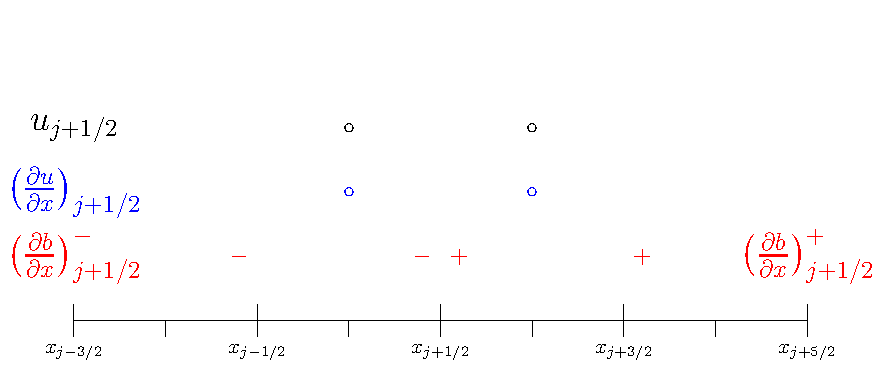
\includegraphics[width=0.8\textwidth]{./chp3/figures/2ndorderrecon.pdf}
	\caption{Summary of values necessary to calculate values of interest at cell boundary for the second-order finite difference volume method.}
	\label{fig:2ndorderrecon}
\end{figure}

\subsubsection{Third Order}
For the third-order finite volume method we use the Koren limiter \cite{Koren-B-1993} to reconstruct the cell edges for $h$, $G$ and $b$. For a general quantity $q$ the reconstruction based on the Koren limiter is
\begin{subequations}
	\begin{gather}
	q^-_{j + 1/2} = \bar{q}_j +  \phi^- \left( r_j \right)\left(\bar{q}_j -\bar{q}_{j-1} \right)/2
	\end{gather}
	and
	\begin{gather}
	q^+_{j + 1/2} = \bar{q}_{j+1} - \phi^+ \left(r_{j+1} \right) \left(\bar{q}_{j+1} -\bar{q}_j \right)/2
	\end{gather}
	where
	\begin{gather}
	\phi^-\left(r_j\right) = \max\left[0, \min\left[2 r_j, \dfrac{1 + 2r_j}{3},2\right]\right],
	\end{gather}
	\begin{gather}
	\phi^+\left(r_j\right) = \max\left[0, \min\left[2 r_j, \dfrac{2 + r_j}{3},2\right]\right]
	\end{gather}
	with
	\begin{equation}
	r_j = (\bar{q}_{j+1} - \bar{q}_j )/(\bar{q}_j - \bar{q}_{j-1}).
	\end{equation}
\end{subequations}

While for $u$ the following reconstruction is used

\begin{gather}
u_{j + \frac{1}{2}} = \frac{ - 3u_{j-1}  + 27u_j+ 27u_{j+1} -3u_{j+2} }{48} .
\end{gather}

We approximate the derivatives in the following way

\begin{gather}
\left( \dfrac{\partial b}{\partial x}\right)^-_{j+1/2} = \dfrac{ {b}^-_{j-3/2} - 4 {b}^-_{j-1/2}  + 3 {b}^-_{j+1/2}}{\Delta x},
\end{gather}
\begin{gather}
\left( \dfrac{\partial b}{\partial x}\right)^+_{j+1/2} = \dfrac{3 {b}^+_{j+1/2} + 4 {b}^+_{j+3/2}  -{b}^+_{j+5/2} }{\Delta x},
\end{gather}
\begin{gather}
 \left( \dfrac{\partial u}{\partial x}\right)^-_{j+1/2} = \left( \dfrac{\partial u}{\partial x}\right)^+_{j+1/2} =   \dfrac{ u_{j-1} - 27u_{j} + 27u_{j+1} {-u_{j + 2}} }{24 \Delta x},
\end{gather}

%Comment on upwind/downwin and having different derivative approximations to $u$

\begin{figure}
	\centering
	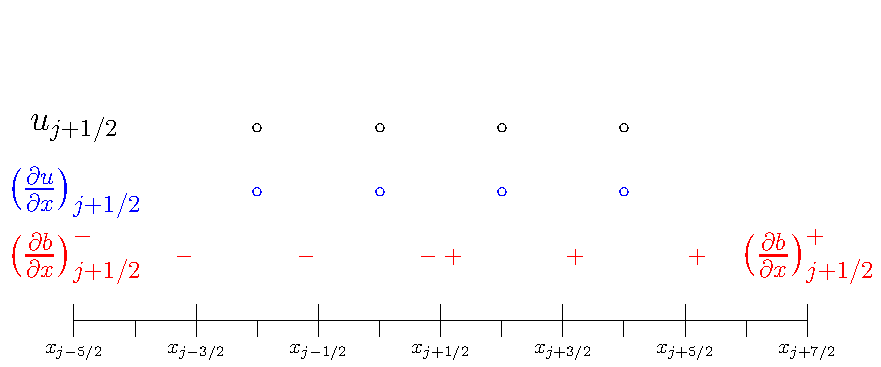
\includegraphics[width=0.8\textwidth]{./chp3/figures/3rdorderecon.pdf}
	\caption{Summary of values necessary to calculate values of interest at cell boundary for the third-order finite difference volume method.}
	\label{fig:3rdorderrecon}
\end{figure}

\subsection{Source Terms and Well Balancing}
%Change this to splitting!
In [] we demonstrated that second-order accuracy is sufficient and so we have only included source terms and well balancing for the second-order method. So this section will only demonstrate the second-order method.

From \eqref{eqn:evolupdatescheme} the only term that we have not computed is $S^n_j$ according to the development of our finite volume method we should have

\begin{equation*}
S^n_j \approx \frac{1}{\Delta t} \int^{t^{n+1}}_{t^n}  \frac{1}{\Delta x}\int^{x_{j+1/2}}_{x_{j-1/2}} S (x,t) dx.
\end{equation*}

Because our time-stepping method for the flux evaluation is only first-order and higher-order temporal schemes are developed using Runge-Kutta steps we can just take the approximation that $S(x,t)$ is constant in time so that

\begin{equation*}
S^n_j \approx \frac{1}{\Delta x}\int^{x_{j+1/2}}_{x_{j-1/2}} S (x,t^n) dx.
\end{equation*}

Where we now only have to ensure that the approximation to the integral of the source term has the appropriate spatial order of accuracy. With the midpoint approximation we have

\begin{equation*}
\frac{1}{\Delta x}\int^{x_{j+1/2}}_{x_{j-1/2}} S (x,t^n) dx = S (x_j,t^n) + \mathcal{O} \left(\Delta x^2\right).
\end{equation*}

So in our second-order method we take

\begin{equation*}
S^n_j = S (x_j,t^n).
\end{equation*}

This means that

\begin{equation}
 S^n_j = -\frac{1}{2}\left(h^n_j\right)^2 {u^n_j}\left( \frac{\partial {u}}{\partial x} \right)^n_j \left(\frac{\partial^2 b}{\partial x^2} \right)^n_j  + h^n_j \left(u^n_j\right)^2 \left(\frac{\partial b}{\partial x}\right)^n_j \left(\frac{\partial^2 b}{\partial x^2}\right)^n_j - gh^n_j\left(\frac{\partial b}{\partial x}\right)^n_j
\end{equation}

where the derivatives and the nodal values must have the appropriate order of accuracy. For the second-order method we already have that the $\bar{h}^n_j =h^n_j$ and $\bar{u}^n_j = u^n_j$ so we turn our attention to the derivatives.  

\subsubsection{Finite Element Method}
In the finite element method we use the polynomial over the cell to approximate the derivative.

For $u$ the quadratic over the cell $\left[x_{j-1/2}, x_{j+1/2}\right]$ is

\begin{equation}
P^u_j(x) = 2\frac{u_{j-1/2} - 2u_{j} + u_{j+1/2}}{\Delta x ^2} \left(x - x_j\right)^2 + \frac{-u_{j-1/2} + u_{j+1/2}}{\Delta x} \left(x - x_j\right) + u_j
\end{equation}

while for $b$ the cubic over the cell is

\begin{multline}
P^b_j(x)= 9\frac{-b_{j-1/2} + 3 b_{j-1/6} - 3 b_{j+1/6} + b_{j+1/2}}{2\Delta x^3} \left(x - x_j\right)^3 \\+  9\frac{b_{j-1/2} - b_{j-1/6} -  b_{j+1/6} + b_{j+1/2}}{4\Delta x^2} \left(x - x_j\right)^2 \\+  \frac{b_{j-1/2} - 27b_{j-1/6} + 27b_{j+1/6} - b_{j+1/2}}{8\Delta x} \left(x - x_j\right) \\  + \frac{1}{16}\left(-b_{j-1/2} + 9 b_{j-1/6} + 9b_{j+1/6} - b_{j+1/2}\right)
\end{multline}

so we have , to make the scheme well balanced we will rely on a slightly different approximation to the bed term that is still second order
\begin{align*}
\left( \frac{\partial {u}}{\partial x} \right)^n_j & = \left. \frac{\partial P^u_j}{\partial x} \right\rvert_{x= x_j} = \frac{-u_{j-1/2} + u_{j+1/2}}{\Delta x} \\
\left( \frac{\partial b}{\partial x} \right)^n_j &  = \left. \frac{\partial P^b_j}{\partial x} \right\rvert_{x= x_j} = \frac{b_{j-1/2} - 27b_{j-1/6} + 27b_{j+1/6} - b_{j+1/2}}{8\Delta x}  \\
\left( \frac{\partial^2 b}{\partial x^2} \right)^n_j & = \left. \frac{\partial^2 P^b_j}{\partial x^2} \right\rvert_{x= x_j} = 9\frac{b_{j-1/2} - b_{j-1/6} -  b_{j+1/6} + b_{j+1/2}}{2\Delta x^2} \\
\end{align*}


\subsubsection{Finite Difference Method}
For the finite difference method we use the following approximations

\begin{align*}
\left( \frac{\partial {u}}{\partial x} \right)^n_j &  = \frac{-u_{j-1/2} +   u_{j+1/2}}{\Delta x} \\
\left( \frac{\partial b}{\partial x} \right)^n_j &  = \frac{-b_{j-1/2} + b_{j+1/2}}{\Delta x}  \\
\left( \frac{\partial^2 b}{\partial x^2} \right)^n_j & = \frac{b_{j-1} - 2b_{j} + b_{j+1}}{\Delta x^2} \\
\end{align*}

\subsubsection{Well balancing}
In [] we demonstrated that the well balancing method of [] for the SWWE can be applied to the Serre equations. To achieve a well balanced method which recovers the lake at rest steady state we use the same method. For completeness we present it here

[]
\begin{alg}
	\label{MethodWellBalancedAudusse}
	\begin{enumerate}
		\item Use the appropriate reconstruction to get the interface values for both $u$ and $G$ giving $u_{i + \frac{1}{2}}$, $G^{-}_{i + \frac{1}{2}}$ and $G^{+}_{i + \frac{1}{2}}$.
		\item Use the second order reconstruction to get the interface values for $h+b$ and $h$ giving $(h+b)^{-}_{i + \frac{1}{2}}$, $(h+b)^{+}_{i + \frac{1}{2}}$, $h^{-}_{i + \frac{1}{2}}$ and $h^{+}_{i + \frac{1}{2}}$.
		\item Calculate the interface values for $b$ by using the reconstructed values of $h+b$ and $h$ above by simply taking the difference giving $b^{-}_{i + \frac{1}{2}}$ and $b^{+}_{i + \frac{1}{2}}$.
		\item Define $\acute{b}_{i + \frac{1}{2}} = \max\left(b^{-}_{i + \frac{1}{2}} , b^{+}_{i + \frac{1}{2}}\right)$
		\item Define $\acute{h}^{-}_{i + \frac{1}{2}} = \max\left(0 ,(h+b)^{-}_{i + \frac{1}{2}} - \acute{b}_{i + \frac{1}{2}} \right)$ and $\acute{h}^{+}_{i + \frac{1}{2}} = \max\left(0 ,(h+b)^{+}_{i + \frac{1}{2}} - \acute{b}_{i + \frac{1}{2}} \right)$
		\item Calculate the flux as in chapter \ref{chapter4} at $x_{i + \frac{1}{2}}$ using $\acute{U}^{+}_{i + \frac{1}{2}} = \left(\begin{array}{c}
		\acute{h}^{+}_{i + \frac{1}{2}} \\
		H^+_{i + \frac{1}{2}}
		\end{array}\right)$ and $\acute{U}^{-}_{i + \frac{1}{2}} = \left(\begin{array}{c}
		\acute{h}^{-}_{i + \frac{1}{2}} \\
		H^-_{i + \frac{1}{2}}
		\end{array}\right)$ as the conserved variables on the right and left respectively. With the $u^{+}_{i + \frac{1}{2}}$ and $b^{+}_{i + \frac{1}{2}}$ giving the right velocity and bed. While $u^{-}_{i + \frac{1}{2}}$ and $b^{-}_{i + \frac{1}{2}}$ gives the left velocity and bed.
		\item Repeat for the other boundary at $x_{i - \frac{1}{2}}$ 
		\item Calculate the source term $S_{ci}$ 
		\[S_{ci} = \Delta x \left(\begin{array}{c}
		0 \\
		-g h \frac{\partial b}{\partial x} - \frac{1}{2} h^2 {u} \frac{\partial {u}}{\partial x} \frac{\partial^2 b}{\partial x^2} + h {u}^2 \frac{\partial b}{\partial x} \frac{\partial^2 b}{\partial x^2}
		\end{array}\right)\]
		by the appropriate method given above, with the following modification
		\begin{equation*}
		\frac{\partial b}{\partial x} = \frac{  - b^{+}_{i - \frac{1}{2}} + b^{-}_{i + \frac{1}{2}}}{\Delta x}\\
		\end{equation*}
		\item Calculate the corrective source term $S_{bi}$ where $S_{bi} = S^{-}_{i + \frac{1}{2}} + S^{+}_{i - \frac{1}{2}}$
		%  
		\[S^{-}_{i + \frac{1}{2}} = \left(\begin{array}{c} 0 \\ \frac{g}{2} \left(\acute{h}^{-}_{i + \frac{1}{2}} \right)^2 - \frac{g}{2} \left(h^{-}_{i + \frac{1}{2}} \right)^2  \end{array}\right) \]
		\[S^{+}_{i - \frac{1}{2}} = \left(\begin{array}{c} 0 \\ \frac{g}{2} \left(h^{+}_{i - \frac{1}{2}}\right)^2 - \frac{g}{2}\left(\acute{h}^{+}_{i - \frac{1}{2}}\right)^2  \end{array}\right) \]
		%
		\item Update according to \eqref{eqnFVMconservationlawupdateformulafix} with the original average values for $U_i$ and the calculated values for the fluxes and $S_i = S_{bi} + S_{ci}$
	\end{enumerate}
\end{alg}

\section{Runge-Kutta Time-Stepping}
The method $\mathcal{E}$ is only first order in time, one strategy for increasing our order of accuracy in time is to use SSP Runge Kutta time stepping []. 

For the first order method our current method is sufficient and so

\begin{equation}
\bar{\boldsymbol{h}}^{n+1} , \bar{\boldsymbol{G}}^{n + 1} = \mathcal{E} \left(\bar{\boldsymbol{h}}^{n} , \bar{\boldsymbol{G}}^{n} , \boldsymbol{b}\right)
\end{equation}

For the second order method we have

\begin{subequations}
\begin{equation}
\bar{\boldsymbol{h}}' , \bar{\boldsymbol{G}}' = \mathcal{E} \left(\bar{\boldsymbol{h}}^{n} , \bar{\boldsymbol{G}}^{n} , \boldsymbol{b}\right)
\end{equation}

\begin{equation}
\bar{\boldsymbol{h}}'' , \bar{\boldsymbol{G}}'' = \mathcal{E} \left(\bar{\boldsymbol{h}}' , \bar{\boldsymbol{G}}' , \boldsymbol{b}\right)
\end{equation}

\begin{equation}
\bar{\boldsymbol{h}}^{n+1} , \bar{\boldsymbol{G}}^{n+1} =  \frac{1}{2} \left(\bar{\boldsymbol{h}}^{n} +\bar{\boldsymbol{h}}'' \right),  \frac{1}{2} \left(\bar{\boldsymbol{G}}^{n} +\bar{\boldsymbol{G}}'' \right)
\end{equation}
\end{subequations}

For the third order method we have

\begin{subequations}
	\begin{equation}
	\bar{\boldsymbol{h}}' , \bar{\boldsymbol{G}}' = \mathcal{E} \left(\bar{\boldsymbol{h}}^{n} , \bar{\boldsymbol{G}}^{n} , \boldsymbol{b}\right)
	\end{equation}
	
	\begin{equation}
	\bar{\boldsymbol{h}}'' , \bar{\boldsymbol{G}}'' = \mathcal{E} \left(\bar{\boldsymbol{h}}' , \bar{\boldsymbol{G}}' , \boldsymbol{b}\right)
	\end{equation}
	
	\begin{equation}
	\bar{\boldsymbol{h}}''' , \bar{\boldsymbol{G}}''' =  \frac{3}{4} \bar{\boldsymbol{h}}^{n} + \frac{1}{4}\bar{\boldsymbol{h}}'' ,  \frac{3}{4} \bar{\boldsymbol{G}}^{n} + \frac{1}{4}\bar{\boldsymbol{G}}''
	\end{equation}
	
	\begin{equation}
	\bar{\boldsymbol{h}}'''' , \bar{\boldsymbol{G}}'''' =  \mathcal{E} \left(\bar{\boldsymbol{h}}''' , \bar{\boldsymbol{G}}''' , \boldsymbol{b}\right)
	\end{equation}
	
	\begin{equation}
	\bar{\boldsymbol{h}}^{n+1}, \bar{\boldsymbol{G}}^{n+1} =  \frac{1}{3} \bar{\boldsymbol{h}}^{n} + \frac{2}{3}\bar{\boldsymbol{h}}'''' ,  \frac{1}{3} \bar{\boldsymbol{G}}^{n} + \frac{2}{3}\bar{\boldsymbol{G}}''''
	\end{equation}
\end{subequations}

\section{CFL Condition}
